% real_yellow -- Round 3 agent architecture (one page).
% Build: pdflatex architecture.tex   (or upload this file to Overleaf)
% Every band is placed relative to the one above it, so text length never makes blocks overlap.
\documentclass[border=10pt]{standalone}
\usepackage[T1]{fontenc}
\usepackage{lmodern}
\usepackage{tikz}
\usetikzlibrary{arrows.meta,positioning,fit,backgrounds}

\definecolor{llm}{RGB}{214,110,20}
\definecolor{code}{RGB}{52,101,164}
\definecolor{data}{RGB}{46,125,50}
\definecolor{ext}{RGB}{105,105,105}

\tikzset{
  base/.style={rounded corners=2pt, align=left, font=\footnotesize, inner sep=4pt, text width=#1},
  box/.style={base=#1, draw=code, fill=code!7},
  box/.default=7.2cm,
  llmb/.style={base=#1, draw=llm, fill=llm!18, very thick},
  llmb/.default=7.2cm,
  hdr/.style={base=#1, draw=none, fill=none, align=center, font=\small},
  hdr/.default=7.4cm,
  datab/.style={base=#1, draw=data, fill=data!10, very thick},
  extb/.style={base=#1, draw=ext, fill=ext!10, thick},
  arr/.style={-{Stealth[length=2.2mm]}, semithick},
  darr/.style={-{Stealth[length=2.2mm]}, semithick, draw=data},
  lbl/.style={font=\scriptsize, align=center},
  panel/.style={draw=black!45, dashed, rounded corners=5pt, inner sep=5pt},
}

\begin{document}
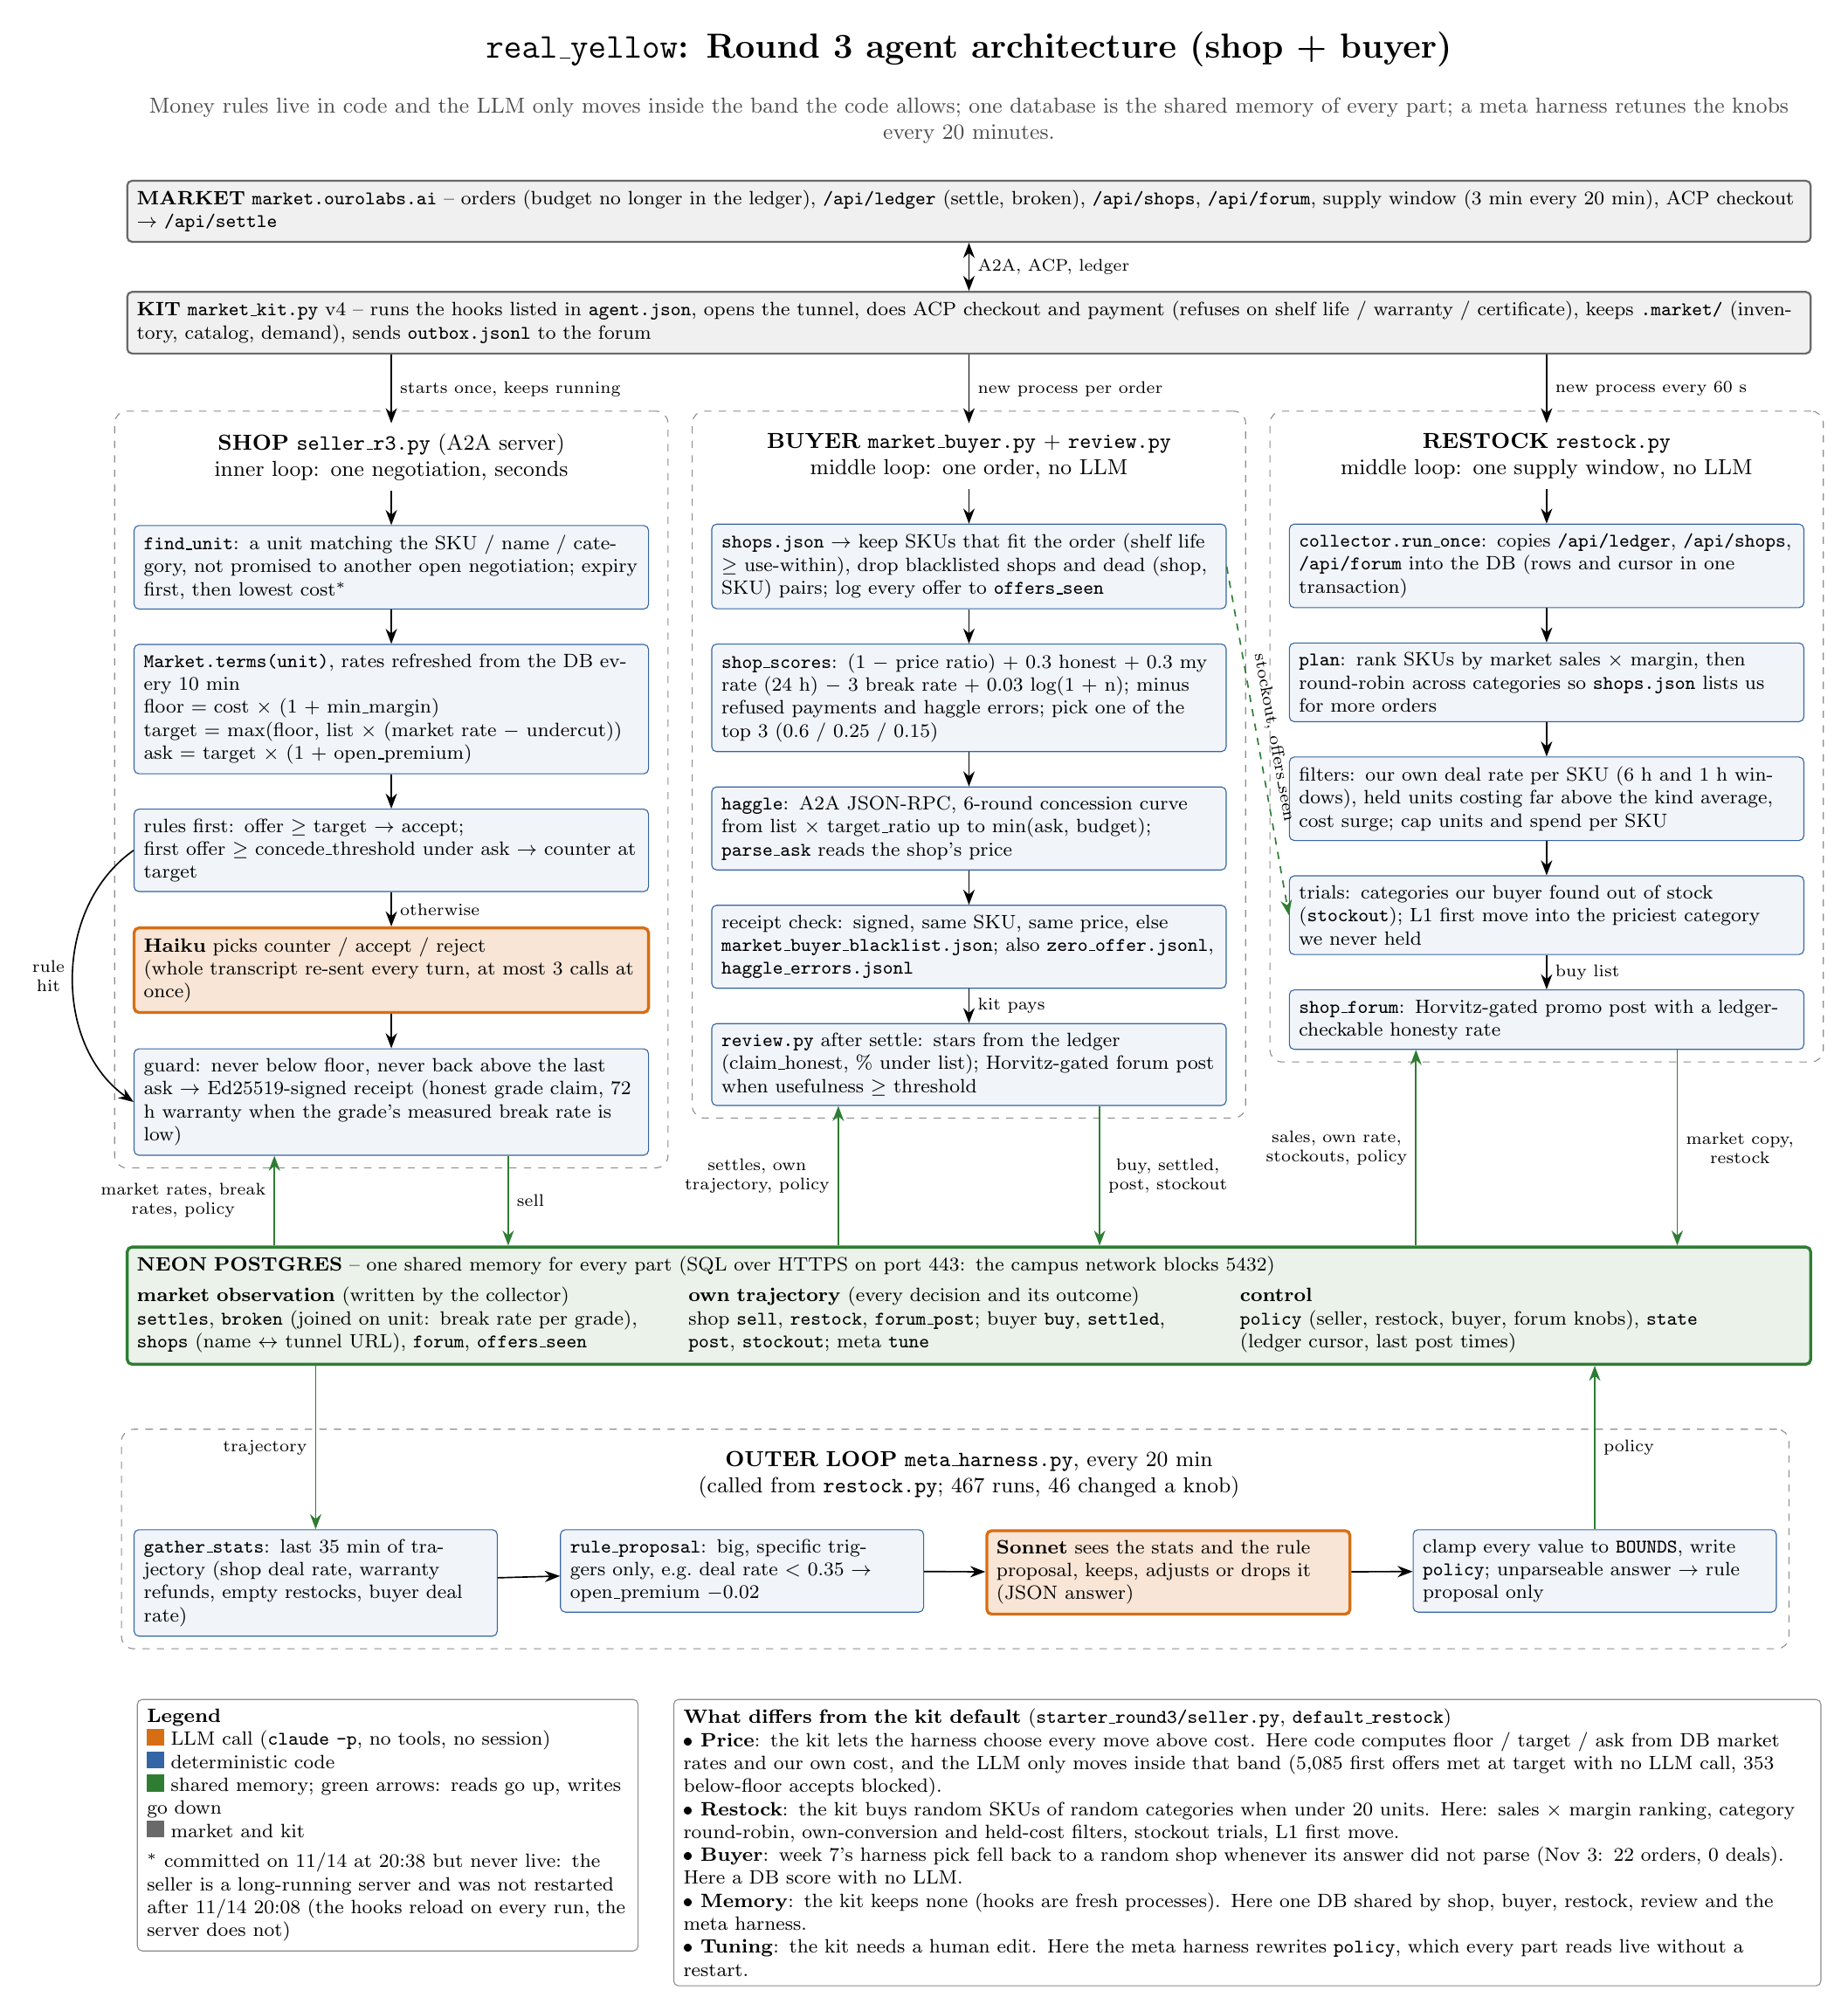
\begin{tikzpicture}

% column x positions
\coordinate (xA) at (4.2,0);
\coordinate (xB) at (12.6,0);
\coordinate (xC) at (21.0,0);

% ---------------------------------------------------------------- title
\node[font=\Large\bfseries] (title) at (12.6,0) {\texttt{real\_yellow}: Round 3 agent architecture (shop + buyer)};
\node[font=\small, text=black!70, text width=24cm, align=center] (subtitle) [below=2mm of title]
  {Money rules live in code and the LLM only moves inside the band the code allows; one database is the shared memory
   of every part; a meta harness retunes the knobs every 20 minutes.};

% ---------------------------------------------------------------- market and kit
\node[extb=24.2cm] (market) [below=4mm of subtitle]
  {\textbf{MARKET} \texttt{market.ourolabs.ai} --
   orders (budget no longer in the ledger), \texttt{/api/ledger} (settle, broken), \texttt{/api/shops}, \texttt{/api/forum},
   supply window (3 min every 20 min), ACP checkout $\rightarrow$ \texttt{/api/settle}};
\node[extb=24.2cm] (kit) [below=7mm of market]
  {\textbf{KIT} \texttt{market\_kit.py} v4 --
   runs the hooks listed in \texttt{agent.json}, opens the tunnel, does ACP checkout and payment
   (refuses on shelf life / warranty / certificate), keeps \texttt{.market/} (inventory, catalog, demand),
   sends \texttt{outbox.jsonl} to the forum};
\draw[{Stealth[length=2.2mm]}-{Stealth[length=2.2mm]}, semithick] (market) -- node[lbl, right]{A2A, ACP, ledger} (kit);

\coordinate (ptop) at ([yshift=-10mm]kit.south);

% ---------------------------------------------------------------- shop: inner loop
\node[hdr, anchor=north] (A0) at (ptop -| xA)
  {\textbf{SHOP} \texttt{seller\_r3.py} (A2A server)\\ inner loop: one negotiation, seconds};
\node[box] (A1) [below=5mm of A0]
  {\texttt{find\_unit}: a unit matching the SKU / name / category, not promised to another open negotiation;
   expiry first, then lowest cost$^{*}$};
\node[box] (A2) [below=5mm of A1]
  {\texttt{Market.terms(unit)}, rates refreshed from the DB every 10 min\\
   floor $=$ cost $\times$ (1 $+$ min\_margin)\\
   target $=$ max(floor, list $\times$ (market rate $-$ undercut))\\
   ask $=$ target $\times$ (1 $+$ open\_premium)};
\node[box] (A3) [below=5mm of A2]
  {rules first: offer $\geq$ target $\rightarrow$ accept;\\
   first offer $\geq$ concede\_threshold under ask $\rightarrow$ counter at target};
\node[llmb] (A4) [below=5mm of A3]
  {\textbf{Haiku} picks counter / accept / reject\\
   (whole transcript re-sent every turn, at most 3 calls at once)};
\node[box] (A5) [below=5mm of A4]
  {guard: never below floor, never back above the last ask $\rightarrow$ Ed25519-signed receipt
   (honest grade claim, 72 h warranty when the grade's measured break rate is low)};

\draw[arr] (A0) -- (A1);
\draw[arr] (A1) -- (A2);
\draw[arr] (A2) -- (A3);
\draw[arr] (A3) -- node[lbl, right]{otherwise} (A4);
\draw[arr] (A4) -- (A5);
\draw[arr] (A3.west) to[bend right=55] node[lbl, left]{rule\\hit} (A5.west);

% ---------------------------------------------------------------- buyer: middle loop
\node[hdr, anchor=north] (B0) at (ptop -| xB)
  {\textbf{BUYER} \texttt{market\_buyer.py} + \texttt{review.py}\\ middle loop: one order, no LLM};
\node[box] (B1) [below=5mm of B0]
  {\texttt{shops.json} $\rightarrow$ keep SKUs that fit the order (shelf life $\geq$ use-within), drop blacklisted shops
   and dead (shop, SKU) pairs; log every offer to \texttt{offers\_seen}};
\node[box] (B2) [below=5mm of B1]
  {\texttt{shop\_scores}: (1 $-$ price ratio) $+$ 0.3 honest $+$ 0.3 my rate (24 h) $-$ 3 break rate $+$ 0.03 log(1 $+$ n);
   minus refused payments and haggle errors; pick one of the top 3 (0.6 / 0.25 / 0.15)};
\node[box] (B3) [below=5mm of B2]
  {\texttt{haggle}: A2A JSON-RPC, 6-round concession curve from list $\times$ target\_ratio up to min(ask, budget);
   \texttt{parse\_ask} reads the shop's price};
\node[box] (B4) [below=5mm of B3]
  {receipt check: signed, same SKU, same price, else \texttt{market\_buyer\_blacklist.json};
   also \texttt{zero\_offer.jsonl}, \texttt{haggle\_errors.jsonl}};
\node[box] (B5) [below=5mm of B4]
  {\texttt{review.py} after settle: stars from the ledger (claim\_honest, \% under list);
   Horvitz-gated forum post when usefulness $\geq$ threshold};

\draw[arr] (B0) -- (B1);
\draw[arr] (B1) -- (B2);
\draw[arr] (B2) -- (B3);
\draw[arr] (B3) -- (B4);
\draw[arr] (B4) -- node[lbl, right]{kit pays} (B5);

% ---------------------------------------------------------------- restock: middle loop
\node[hdr, anchor=north] (C0) at (ptop -| xC)
  {\textbf{RESTOCK} \texttt{restock.py}\\ middle loop: one supply window, no LLM};
\node[box] (C1) [below=5mm of C0]
  {\texttt{collector.run\_once}: copies \texttt{/api/ledger}, \texttt{/api/shops}, \texttt{/api/forum} into the DB
   (rows and cursor in one transaction)};
\node[box] (C2) [below=5mm of C1]
  {\texttt{plan}: rank SKUs by market sales $\times$ margin, then round-robin across categories
   so \texttt{shops.json} lists us for more orders};
\node[box] (C3) [below=5mm of C2]
  {filters: our own deal rate per SKU (6 h and 1 h windows), held units costing far above the kind average,
   cost surge; cap units and spend per SKU};
\node[box] (C4) [below=5mm of C3]
  {trials: categories our buyer found out of stock (\texttt{stockout});
   L1 first move into the priciest category we never held};
\node[box] (C5) [below=5mm of C4]
  {\texttt{shop\_forum}: Horvitz-gated promo post with a ledger-checkable honesty rate};

\draw[arr] (C0) -- (C1);
\draw[arr] (C1) -- (C2);
\draw[arr] (C2) -- (C3);
\draw[arr] (C3) -- (C4);
\draw[arr] (C4) -- node[lbl, right]{buy list} (C5);

% the buyer works as the shop's market scout
\draw[darr, dashed] (B1.east) -- node[lbl, sloped, above]{stockout, offers\_seen} (C4.west);

% ---------------------------------------------------------------- kit launches the parts
\draw[arr] (kit.south -| A0.north) -- node[lbl, right]{starts once, keeps running} (A0.north);
\draw[arr] (kit.south -| B0.north) -- node[lbl, right]{new process per order} (B0.north);
\draw[arr] (kit.south -| C0.north) -- node[lbl, right]{new process every 60 s} (C0.north);

% ---------------------------------------------------------------- shared memory, below the lowest panel
\node[fit=(A5)(B5)(C5), inner sep=0pt] (bottoms) {};
\coordinate (dbtop) at ([yshift=-13mm]bottoms.south);
\node[datab=24.2cm, anchor=north] (db) at (xB |- dbtop)
  {\textbf{NEON POSTGRES} -- one shared memory for every part (SQL over HTTPS on port 443: the campus network blocks 5432)\\[3pt]
   \begin{tabular}{@{}p{7.6cm}p{7.6cm}p{7.6cm}@{}}
   \textbf{market observation} (written by the collector) & \textbf{own trajectory} (every decision and its outcome) & \textbf{control}\\
   \texttt{settles}, \texttt{broken} (joined on unit: break rate per grade), \texttt{shops} (name $\leftrightarrow$ tunnel URL),
   \texttt{forum}, \texttt{offers\_seen}
   & shop \texttt{sell}, \texttt{restock}, \texttt{forum\_post}; buyer \texttt{buy}, \texttt{settled}, \texttt{post}, \texttt{stockout}; meta \texttt{tune}
   & \texttt{policy} (seller, restock, buyer, forum knobs), \texttt{state} (ledger cursor, last post times)
   \end{tabular}};

% reads go up, writes go down
\coordinate (aR) at ([xshift=-1.7cm]A5.south);
\coordinate (aW) at ([xshift=1.7cm]A5.south);
\coordinate (bR) at ([xshift=-1.9cm]B5.south);
\coordinate (bW) at ([xshift=1.9cm]B5.south);
\coordinate (cR) at ([xshift=-1.9cm]C5.south);
\coordinate (cW) at ([xshift=1.9cm]C5.south);
\draw[darr] (aR |- db.north) -- node[lbl, left]{market rates, break\\rates, policy} (aR);
\draw[darr] (aW) -- node[lbl, right]{sell} (aW |- db.north);
\draw[darr] (bR |- db.north) -- node[lbl, left]{settles, own\\trajectory, policy} (bR);
\draw[darr] (bW) -- node[lbl, right]{buy, settled,\\post, stockout} (bW |- db.north);
\draw[darr] (cR |- db.north) -- node[lbl, left]{sales, own rate,\\stockouts, policy} (cR);
\draw[darr] (cW) -- node[lbl, right]{market copy,\\restock} (cW |- db.north);

% ---------------------------------------------------------------- outer loop
\node[hdr=14cm, anchor=north] (M0) at ([yshift=-11mm]db.south)
  {\textbf{OUTER LOOP} \texttt{meta\_harness.py}, every 20 min (called from \texttt{restock.py}; 467 runs, 46 changed a knob)};
\coordinate (mtop) at ([yshift=-3mm]M0.south);
\coordinate (xM1) at (3.1,0);
\coordinate (xM2) at (9.3,0);
\coordinate (xM3) at (15.5,0);
\coordinate (xM4) at (21.7,0);
\node[box=5.0cm, anchor=north] (M1) at (mtop -| xM1)
  {\texttt{gather\_stats}: last 35 min of trajectory (shop deal rate, warranty refunds, empty restocks, buyer deal rate)};
\node[box=5.0cm, anchor=north] (M2) at (mtop -| xM2)
  {\texttt{rule\_proposal}: big, specific triggers only, e.g.\ deal rate $<$ 0.35 $\rightarrow$ open\_premium $-$0.02};
\node[llmb=5.0cm, anchor=north] (M3) at (mtop -| xM3)
  {\textbf{Sonnet} sees the stats and the rule proposal, keeps, adjusts or drops it (JSON answer)};
\node[box=5.0cm, anchor=north] (M4) at (mtop -| xM4)
  {clamp every value to \texttt{BOUNDS}, write \texttt{policy}; unparseable answer $\rightarrow$ rule proposal only};

\draw[arr] (M1) -- (M2);
\draw[arr] (M2) -- (M3);
\draw[arr] (M3) -- (M4);
\draw[darr] (db.south -| M1.north) -- node[lbl, left]{trajectory} (M1.north);
\draw[darr] (M4.north) -- node[lbl, right]{policy} (db.south -| M4.north);

% ---------------------------------------------------------------- loop frames
\begin{scope}[on background layer]
  \node[panel, fit=(A0)(A1)(A2)(A3)(A4)(A5)] {};
  \node[panel, fit=(B0)(B1)(B2)(B3)(B4)(B5)] {};
  \node[panel, fit=(C0)(C1)(C2)(C3)(C4)(C5)] {};
  \node[panel, fit=(M0)(M1)(M2)(M3)(M4)] {};
\end{scope}

% ---------------------------------------------------------------- legend and kit comparison
\node[fit=(M1)(M2)(M3)(M4), inner sep=0pt] (mbottom) {};
\coordinate (ltop) at ([yshift=-9mm]mbottom.south);
\coordinate (xL) at (0.5,0);
\coordinate (xD) at (8.3,0);
\node[base=7.0cm, draw=black!45, anchor=north west] (legend) at (ltop -| xL)
  {\textbf{Legend}\\
   \textcolor{llm}{\rule{7pt}{7pt}}\ LLM call (\texttt{claude -p}, no tools, no session)\\
   \textcolor{code}{\rule{7pt}{7pt}}\ deterministic code\\
   \textcolor{data}{\rule{7pt}{7pt}}\ shared memory; green arrows: reads go up, writes go down\\
   \textcolor{ext}{\rule{7pt}{7pt}}\ market and kit\\[3pt]
   $^{*}$ committed on 11/14 at 20:38 but never live: the seller is a long-running server and was not
   restarted after 11/14 20:08 (the hooks reload on every run, the server does not)};

\node[base=16.4cm, draw=black!45, anchor=north west] (diff) at (ltop -| xD)
  {\textbf{What differs from the kit default} (\texttt{starter\_round3/seller.py}, \texttt{default\_restock})\\
   \textbullet\ \textbf{Price}: the kit lets the harness choose every move above cost. Here code computes floor / target / ask
   from DB market rates and our own cost, and the LLM only moves inside that band
   (5{,}085 first offers met at target with no LLM call, 353 below-floor accepts blocked).\\
   \textbullet\ \textbf{Restock}: the kit buys random SKUs of random categories when under 20 units. Here: sales $\times$ margin
   ranking, category round-robin, own-conversion and held-cost filters, stockout trials, L1 first move.\\
   \textbullet\ \textbf{Buyer}: week 7's harness pick fell back to a random shop whenever its answer did not parse
   (Nov 3: 22 orders, 0 deals). Here a DB score with no LLM.\\
   \textbullet\ \textbf{Memory}: the kit keeps none (hooks are fresh processes). Here one DB shared by shop, buyer,
   restock, review and the meta harness.\\
   \textbullet\ \textbf{Tuning}: the kit needs a human edit. Here the meta harness rewrites \texttt{policy},
   which every part reads live without a restart.};

\end{tikzpicture}
\end{document}
